% chap5.tex (Methodology and Result)

\chapter{Methodology and Results}

In this chapter, I describe the methodologies I have followed to find answers of the research questions I have described in Chapter 1.


\section{Learning Algorithms, Train and Test Set}
I have tried several learning algorithms that are available in Weka \cite{witten2005data}. I was looking for learning algorithms that can be trained as quickly as possible with large amount of data and with limited resources. The learning algorithm also has to produce lower error rate and faster output during the time of competition. I have found that M5P, M5RULES, REP TREE, LINEAR REGRESSION \cite{witten2005data} met my requirements. For training the models, I have used 10 game log files. Each log files contain about 10,000 training instances. Training time was taking too long when I was using more than 10 log files. I separated 5 game log files to use as a test set.

\section{The Baseline Electricity Forecasting Mechanisms}
The first baseline energy forecasting mechanism is the default prediction mechanism provided by the PowerTAC system. It exploits the fact that usage of a timeslot of a customer in a specific date is highly correlated with the day of a week and hour of a day. To make a prediction it stores the average energy usage of an hour of a week. So, for each customer, it uses $24*7 = 168$ values to remember average usages. As soon as it informed the new usage information of an hour of a week, it updates old average using the Algorithm \ref{alg:updateAvgMovingAvg}. To make demand forecasts about a customer it uses Algorithm \ref{alg:predictAvgMovingAvg}.

\begin{algorithm}
\caption{Update average usage for $customer_i$ for day d and timeslot t, $newUsage$}
\begin{algorithmic} [1]
\STATE avgUsage = get average usage of $customer_i$ at day d and time slot t
\STATE $avgUsage = 0.7 * avgUsage + 0.3 * newUsage$
\end{algorithmic}
\label{alg:updateAvgMovingAvg}
\end{algorithm}

\begin{algorithm}
\caption{forecast usage for day d and timeslot t for $customer_i$}
\begin{algorithmic} [1]
\STATE avgUsage = get average usage of $customer_i$ at day d and time slot t 
\STATE return $avgUsage$
\end{algorithmic}
 \label{alg:predictAvgMovingAvg}
\end{algorithm}

\section{Single Demand Predictor}
All the activities that occurred in a game can be found in a game log.  Activities such as buying or selling electricity occur during a time slot. At the beginning of a time slot, the system notifies the broker that a new time slot is about to begin. The system also notifies the brokers with weather forecast about the future time slots. As a time slot ends, the broker receives information about its customer's energy usage which is called tariff transaction report. Algorithm \ref{alg:ttxHandle} specifies how the extraction program retrieves the necessary information from the tariff transaction report. As the broker gets notification of the beginning of a new time slot, the extraction program has all the information related to energy usage and weather data of the previous time slot available by this time. I started with a large number of features at the beginning. The features included time related features such as day of week, hour of day, month of year; weather related features such as cloud cover, wind speed, temperature; historical data such as last past 24 slot's electricity usage, last week's electricity usage and statistical features such as average and standard deviation of the weekly slot. Algorithm \ref{algo:bestSingle} shows how a single prediction model is created. It can be seen that the training set had information about all the customers of all types discussed in Chapter 3. For this scheme the baseline predictor produced on average 70\% root relative percentage error. And for all learning algorithms, the error rate was more than 80\%. The reason behind this poor perfomance is irregularity in training data. As we saw earlier, not all customers have regularity in their electricity usage pattern. As I have aggregated information about all the customers, which included irregularity, the training model might not be able to generalize knowledge from the training set properly. 

%feature extraction
\begin{algorithm}[!h]
\caption{extract information from transactionReport sent to broker after each time slot through TariffTransactionHandler call back method}
\begin{algorithmic} [1]
\STATE timeSlot = get time slot from transactionReport
\STATE customerName = get customer name from transactionReport
\STATE energyUsed = get energy used from trom transactionReport
\STATE addUsage(customerName, timeSlot, energyUsed)
\end{algorithmic}
 \label{alg:ttxHandle}
\end{algorithm}

%write extracted features
\begin{algorithm} [!h]
\caption{write extracted data after timeSlot update message received from TimeSlotUpdateHandler call back method}
\begin{algorithmic} [1]
\STATE knownTimeSlot = timeSlot - 1
\FOR{each customer}
\STATE day = get day of knownTimeSlot
\STATE hour = get hour of knownTimeSlot
\STATE statisticalData = get statistics of the customer of day and hour
\STATE weatherData = get weather data of knownTimeSlot
\STATE trueUsage = get true usage of customer in knownTimeSlot
\STATE trainingInstance = create training instance by combining statistical data, weather data and true usage 
\STATE writeToFile(trainingInstance)
\ENDFOR
\end{algorithmic}
\label{alg:writeSlotInfo}
\end{algorithm}

%find best performing single prediction model
%find best classifier for individual customers
\begin{algorithm}[!h]
\caption{find a single best classifier}
\begin{algorithmic} [1]
\STATE combine all slot based training instance of all the customers
\STATE train available classifiers on the combined data using 10 fold cross validation
\STATE choose the classifier with minimum error
\STATE save the classifier for making prediction about all the customers
\end{algorithmic}
\label{alg:bestSingle}
\end{algorithm}

\section{Individual Demand Predictor}

From the experience of a single demand predictor, I included only information about consumption customer data in training set. So the training set no longer had information about interruptible consumption, thermal storage or electric vehicle. Also, this time the feature was reduced using Weka's attribute selection algorithm \cite{witten2005data}. Out of 54 features, only 5 were choosen. The features were temperature, wind speed, cloud cover, average of the weekly hour slot, standard deviation of the weekly hour slot. Features extracted for each customer served as a separated training data set. I trained an individual predictor model for each customer model. In general, if there are n customers in the system, we will need n electricity demand predictors each one trained on the data of a single customer. I went further by checking different machine learning algorithms such as M5Tree \cite{witten2005data}, Linear Regression \cite{witten2005data}, M5P rules \cite{witten2005data} and REP tree \cite{witten2005data} for each customer and picking the best performing one for each customer. The process of finding best prediction model for each customer is shown in Algorithm \ref{alg:bestClassifierForCluster}. Each prediction model will make electricity load demand prediction for each customer. Broker will know the electricity demand by summing over all the predictions.

\begin{algorithm}[!h]
\caption{find best classifiers created for each individual customer}
\begin{algorithmic} [1]
\FOR{each customer}
    \STATE combine all slot based training instance of the customer
    \STATE train available classifiers on the combined data using 10 fold cross validation
    \STATE choose the classifier with minimum error
    \STATE save the classifier for making prediction about the customer
\ENDFOR 
\end{algorithmic}
\label{alg:bestClassifierIndiv}
\end{algorithm}


\section{Cluster Based Demand Predictor}
One problem with the individual demand predictor is that it this system has a demand prediction model for each known customer. So, it cannot make demand forecasts for a novel customer. This is a serious problem because during a competition the system may introduce a new customer or change name of a customer. In those cases the individual demand prediction mechanism becomes unreliable. To mitigate this issue, I proposed a solution that groups the customer based on their weekly average usage. Algorithm \ref{alg:writeWeeklyAvg} shows the procedure for extracting average electricity usage of each hour of a week. Next, all the average weekly usages are combined together to make training set for the clustering algorithm. I have used k-means \cite{witten2005data} clustering algorithm to cluster the  training set. I have trained clusters of sizes 4, 5, 6, 7, 8, 9, 10 and 11. Algorithm \ref{alg:makeCluster} describes the procedure for making clusters from the training instances. Once a k-means of cluster size k is made, a program groups the hourly usages of the customers in the same cluster and combines them to make training set for  machine learning classifier. This training set is used to train linear regression classifier. Algorithm \ref{alg:errorOfCluster} describes how the cluster based predictor's performance was evaluated.
%observe error of each cluster
Based on the errors observed from different k-means cluster based forecasting mechanisms, I fixed the number of clusters. Once the number of the clusters was fixed, a program creates several machine learning predictors to see which one performs best for a given cluster. The machine learning classifiers that were tried out are linear regression \cite{witten2005data}, M5P rules \cite{witten2005data}, M5 Tree\cite{witten2005data}, REP tree\cite{witten2005data}. At runtime, a customer will be grouped in a cluster based on its weekly usage. Once the program knows the cluster assigned to a customer, the program will load the corresponding demand forecaster to make electricity demand forecast about the customers.

\begin{algorithm} [!h]
\caption{write average electricity usage of the customers of each hour of the week}
\begin{algorithmic} [1]
\REQUIRE information of all timeslots has been received
\FOR{each customer}
    \STATE trainingInstance = create empty training instance
    \FOR{each day of week}
        \FOR{each hour of day}
            \STATE averageUsage = get average usage of day and hour of customer
            \STATE append averageUsage to the trainingInstance
        \ENDFOR
    \ENDFOR
    \STATE writeToAvgUsageFile(trainingInstance)
\ENDFOR
\end{algorithmic}
\label{alg:writeWeeklyAvg}
\end{algorithm}

%make cluster

\begin{algorithm}
\caption{create kmeans cluster of size k from weekly usage training instance file}
\begin{algorithmic} [1]
\STATE data = load weekly average usage file
\STATE kmeansCluster = build kmeans cluster of size k based on data
\STATE save kmeansCluster
\end{algorithmic}
\label{alg:makeCluster}
\end{algorithm}

%find size of k
\begin{algorithm}[!h]
\caption{find error of kmeans clusters of different size}
\begin{algorithmic} [1]

\FOR{each cluster size k}
    \STATE get the kMeansCluster of size k
    \FOR{cluster in KMeansCluster}
        \STATE combine slot based training instances of that cluster
        \STATE train linear regression classifier based on the combined data
        \STATE save the classifier for cluster
    \ENDFOR
\ENDFOR

\FOR{each training instance}
    \STATE compute error of the instance using each kMeansCluster
\ENDFOR
\end{algorithmic}
\label{alg:errorOfCluster}
\end{algorithm}

%find best classifier for cluster of size k
\begin{algorithm} [!h]
\caption{find best classifiers of each cluster of kmeans cluster of size k}
\begin{algorithmic} [1]
\FOR{each cluster in kMeansCluster}
    \STATE combine slot based data of the all the customers in cluster
    \STATE train available classifiers on the combined data using 10 fold cross validation
    \STATE choose the classifier with minimum error
    \STATE save the classifier for making demand forecasting for cluster
\ENDFOR 
\end{algorithmic}
\label{alg:bestClassifierForCluster}
\end{algorithm}

\section{Testing Performance}
Algorithm \ref{alg:performanceEval} shows how accuracy of each prediction model was tested. Each instance of the test set was tested against each demand prediction scheme. Average absoluate percentage error was calculated for each scheme. Algorithm \ref{alg:errorCalculation} shows the algorithm for computing error.
 
%Testing
\begin{algorithm}
\caption{performance evalulation of each method}
\begin{algorithmic} [1]
\FOR{each test instance}
    \STATE classify the test instance using moving average usage \textbf{[algorithm \ref{alg:predictAvgMovingAvg}]}
    \STATE classify the test instance using individual prediction mechanism
    \STATE classify the test instance using cluster based predictor
    \STATE calculate and accumulate errors of each mechanism \textbf{[algorithm\ref{alg:errorCalculation}]}
    \STATE update moving average baseline predictor based on the information from the test instance \textbf{[algorithm \ref{alg:updateAvgMovingAvg}]}
\ENDFOR 
\STATE find average error from the accumulated errors for each forecasting mechanism
\end{algorithmic}
\label{alg:performanceEval}
\end{algorithm}
%calculate error
\begin{algorithm} [!h]
\caption{calculate error from the predicted value and the true value}
\begin{algorithmic} [1]
\STATE absoluteError = abs(predictedValue - trueValue)
\STATE relativeAbsoluteError = (absoluteError / trueValue ) * 100 \%
\end{algorithmic}
\label{alg:errorCalculation}
\end{algorithm}

\section{Experimental Results}

The following subsections describe the results at each stage of experiments. The stages are finding optimal number of clusters. Once the number of clusters has been fixed, different classifier needs to be made for each cluster to see which one makes the best forecast for a particular cluster. After that, the baseline predictor that needs a classifier for each customer needs to be built. At this point, for each customer several classifier has been tried out to see which classifier makes best demand forecast about that customer. After that, the proposed mechanism has been tested against the two baseline demand forecasting methods.

\section{Finding Individual Predictor for Each Customer}
Based on the data from each of the customers, the four types of classifiers described in previously were tried out. For each customer, the Table \ref{table:1} shows the best performing classifier for each customer. 

\begin{table}[h!]
\centering
\caption{Best individual predictor for each customer}
\begin{tabular}{|c| c|} 
 \hline
 Customer Name & Best Predictor Type \\ [0.5ex] 
 \hline
BrooksideHomes &	M5P \\
CentervilleHomes &	M5P \\
DowntownOffices &	M5P \\
EastsideOffices &	M5P \\
OfficeComplex 1 NS Base &	LinearRegression \\
OfficeComplex 1 SS Base &	LinearRegression \\
OfficeComplex 2 NS Base &	LinearRegression \\
OfficeComplex 2 SS Base &	LinearRegression \\
Village 1 NS Base &	M5P \\
Village 1 RaS Base &	LinearRegression \\
Village 1 ReS Base &	M5P \\
Village 1 SS Base &	M5P \\
Village 2 NS Base &	LinearRegression \\
Village 2 RaS Base &	M5P \\
Village 2 ReS Base &	M5P \\
Village 2 SS Base &	M5P \\
MedicalCenter@1	& M5P \\ [1ex] 
 \hline
\end{tabular}
\label{table:1}
\end{table}

The figure \ref{fig:indiv-cutomer-best-predictor-error} shows error percentage of each of the predictors type for each of the customer types.

\begin{figure}[h!]
  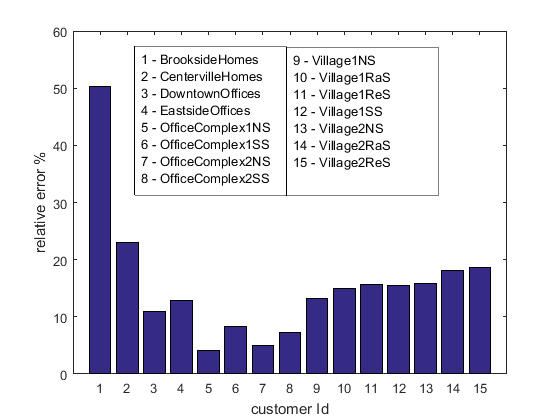
\includegraphics{relativeErrorIndivPredictor.png}
  \caption{Performance of the best classifier for each customer type. Customer Medical center was excluded as it was showing huge error. }
  \label{fig:indiv-cutomer-best-predictor-error}
\end{figure}

%%%%%%%%%%%%%%%%%

\subsection{Finding number of clusters}

At first, I have segmented the customer using KMeans clustering algorithm with cluster sizes = 4, 5, 6, 7, 8, 9, 10 and 11. For kMeans Eucleadian Distance \cite{witten2005data} was used for similarity metric, max number of iteration \cite{witten2005data} was set to 500. For KMeans with size k, we will have k clusters. For each of the k clusters, I had a linear regression predictor. I observed the relative percentage error and absolute average the above cluster sizes. It turned out that the size of the cluster does not have a big impact on the prediction performance. To keep things simple, I have decided to choose Kmeans cluster of size 4. When k = 4 was chosen, table \ref{table:clusterAss} shows the cluster assignment for each customer. It can be seen that, cluster-0 held most of the offices, cluster 2 held most of the village types, cluster 3 held the medical center, cluster 1 held large housing such as brooksidehomes, centerville homes and large offices such as downtown offices and centerville offices.


\begin{table}[h!]
\centering
\caption{Assigned cluster for each customer}
\begin{tabular}{|c| c|} 
 \hline
 Customer Name & Assigned Cluster Number \\ [0.5ex] 
 \hline
BrooksideHomes &	0 \\
CentervilleHomes & 0 \\
DowntownOffices & 1	\\
EastsideOffices &	1 \\
OfficeComplex 1 NS Base &	0 \\
OfficeComplex 1 SS Base &	0 \\
OfficeComplex 2 NS Base &	0 \\
OfficeComplex 2 SS Base &	0 \\
Village 1 NS Base &	2 \\
Village 1 RaS Base &	2 \\
Village 1 ReS Base &	2 \\
Village 1 SS Base &	2 \\
Village 2 NS Base &	2 \\
Village 2 RaS Base &	2 \\
Village 2 ReS Base &	2 \\
Village 2 SS Base &	2 \\
MedicalCenter@1	& 3 \\ [1ex] 
 \hline
\end{tabular}
\label{table:clusterAss}
\end{table}

\subsection {Finding best predictor for each cluster}
Once the features are extracted, I have tried out  M5Tree, Linear Regression, M5P rules and REP tree machine learning classifiers to see which one performs the best for each of the 4 clusters. Figure \ref{fig:cluster-0-predictors}, \ref{fig:cluster-1-predictors}, \ref{fig:cluster-2-predictors}, \ref{fig:cluster-3-predictors} the average relative percentage errors that each classifier produced for cluster 0, 1, 2, and 3 respectively. Figure \ref{fig:cluster-0-predictors} shows that among all the classifiers, M5P produces the minimum amount of error. So M5P will be used as the demand predictor for cluster 0. For cluster 1, 2 and 3 the M5P, REPTREE and M5RULES will be used respectively as demand predictors.

%%trial 1
\begin{figure}
\centering
\begin{minipage}{.5\textwidth}
  \centering
  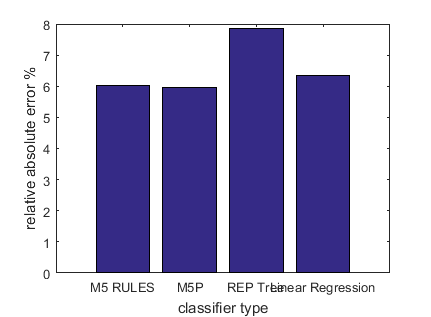
\includegraphics[width=\linewidth]{cluster-0-diff-classifier-relative-abs.png}
  \caption{cluster 0}
  \label{fig:cluster-0-predictors}
\end{minipage}%
\begin{minipage}{.5\textwidth}
  \centering
  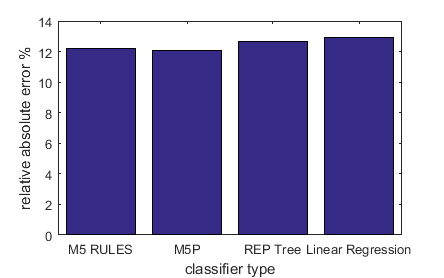
\includegraphics[width=\linewidth]{cluster-1-diff-classifier-relative-abs.png}
  \caption{cluster 1}
\label{fig:cluster-1-predictors}
\end{minipage}

\centering
\begin{minipage}{.5\textwidth}
  \centering
  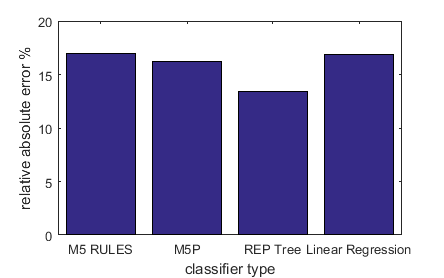
\includegraphics[width=\linewidth]{cluster-2-diff-classifier-relative-abs.png}
  \caption{cluster 2}
  \label{fig:cluster-2-predictors}
\end{minipage}%
\begin{minipage}{.5\textwidth}
  \centering
  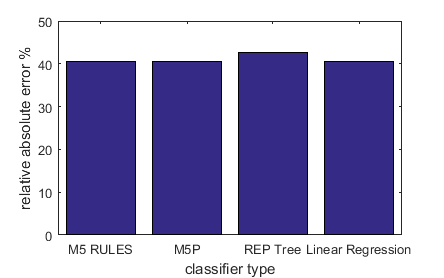
\includegraphics[width=\linewidth]{cluster-3-diff-classifier-relative-abs.png}
  \caption{cluster 3}
\label{fig:cluster-3-predictors}
\end{minipage}

\end{figure}
%% trial 1 end


\subsection{Comparison Among the Three Prediction Schemes}

Finally, all three demand prediction schems were tested with test set. From Figure \ref{fig:prediction-scheme-vs-error}, we can see that cluster based prediction mechanism performed almost as good as the mechanism individual prediction scheme. And it did better than the default moving average prediction scheme.

\begin{figure}[h!]
\centering
\begin{minipage}{.5\textwidth}
  \centering
  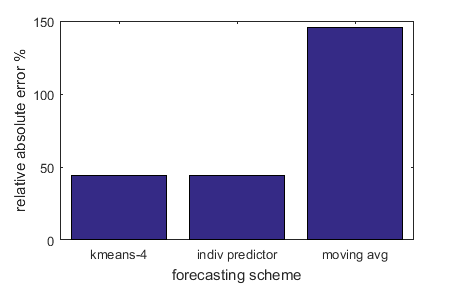
\includegraphics[width=\linewidth]{final-relative-abs-error.png}
  \caption{comparison among three prediction schemes}
  \label{fig:prediction-scheme-vs-error}
\end{minipage}
  
\end{figure}

\subsection{Model Accuracy and Training Set Size}
Figure \ref{fig:trainset-vs-error} shows the error of all three models with increasing training set size. It appears that the accuracy of the models does not change much with increased training set size. The reason behind this reason may be because the models were trained based on past tournament data. May be during a tournament the customer behavior remains unchanged. So adding more data may be redundant. 

\begin{figure}[h!]
\centering
\begin{minipage}{.5\textwidth}
  \centering
  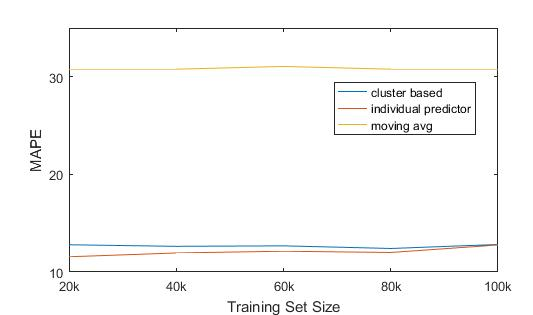
\includegraphics[width=\linewidth]{error-change-training-size.jpg}
  \caption{comparison among three prediction schemes}
  \label{fig:trainset-vs-error}
\end{minipage}
  
\end{figure}